\begin{figure}[H]
    \centering
    \caption{Esquema de uma unidade logística.}
    \label{fig:uni_logistica}
    \scalebox{0.95}{
    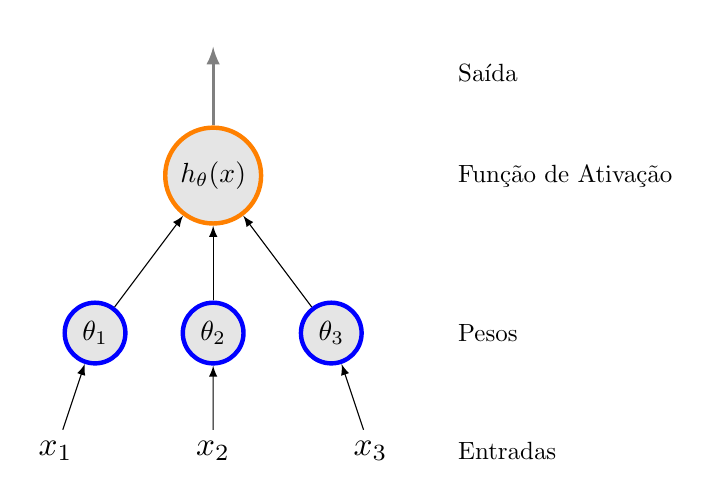
\begin{tikzpicture}
        \tikzstyle{neuronio} = [circle, color=orange, ultra thick, draw, fill=black!10]
    
        \node [neuronio, pin={[pin distance = 10mm, pin edge={-latex, very thick}]above:}] (percep) at (0,0)
        {
        \textcolor{black}{$h_{\bm{\theta}}(\bm{x})$}
        }; % output part ended.
        
        \foreach \i in {1,...,3}
        {
            [level distance = 3cm, sibling distance = 6cm]
            \node [circle, color=blue, ultra thick, draw, fill=black!10] (n-\i) at (\i*1.5-3, -2) {\textcolor{black}{$\theta_{\i}$}};
            \node[scale=1.2] (in-\i) at (\i*2-4, -3.5) {\textcolor{black}{$x_{\i}$}};
        }
        
        \foreach \i in {1,2,3}
        {
            \draw[-latex] (in-\i) -- (n-\i);
            \draw[-latex] (n-\i) -- (percep);
        }
        
        \node[right, scale=0.9] at (3, 1.3) {Saída};
        \node[right, scale=0.9] at (3, 0) {Função de Ativação};
        \node[right, scale=0.9] at (3, -2) {Pesos};
        \node[right, scale=0.9] at (3, -3.5) {Entradas};
    \end{tikzpicture}
    }
    \caption*{\small Fonte: Elaboração própria.}
\end{figure}